\documentclass[11pt]{article}
\usepackage{certmachine}
\usepackage{graphicx}
\usepackage{array}
\newcolumntype{R}[1]{>{\raggedright\arraybackslash}p{#1}}
%% generated by tools/paper-numbers/erdos852.js from certs/erdos852-certificate.json, certs/erdos852-h-records.json, corpus/sources (pinned) — do not edit (git 054078d19462)
\newcommand{\RepoCommit}{054078d19462}
\newcommand{\CertGit}{1d2b452}
\newcommand{\CertSha}{4379194d0bd4}
\newcommand{\CzeroDigitsFull}{1.3232282768639494690289693932974634613586535126004759968489856}
\newcommand{\CzeroDecimals}{61}
\newcommand{\CzeroShort}{1.32322827686394946902}
\newcommand{\CzeroPublished}{1.32322827686395}
\newcommand{\CzeroPubDecimals}{14}
\newcommand{\CzeroBits}{320}
\newcommand{\CzeroBisections}{200}
\newcommand{\CzeroWidthBound}{$7.8\times10^{-62}$}
\newcommand{\CzeroBracketLo}{1.3232282768639494690289693932974634613586}
\newcommand{\CzeroBracketHi}{1.3232282768639494690289693932974634613587}
\newcommand{\CzeroPrefix}{1.32322827686394}
\newcommand{\CzeroContinuation}{9469}
\newcommand{\CzeroRoundedTo}{1.32322827686395}
\newcommand{\CstarLo}{0.0752403861783092455893}
\newcommand{\CstarHi}{0.0752403861783095651674}
\newcommand{\CstarWidth}{$3.20\times10^{-16}$}
\newcommand{\CstarWidthShort}{$3.2\times10^{-16}$}
\newcommand{\CstarDigits}{0.075240386178309}
\newcommand{\CstarAgreedDecimals}{15}
\newcommand{\CstarPrimes}{1{,}857{,}858}
\newcommand{\CstarLimit}{30{,}000{,}000}
\newcommand{\CstarLimitSci}{$3\times10^{7}$}
\newcommand{\CstarBits}{192}
\newcommand{\CstarTail}{$5.56\times10^{-16}$}
\newcommand{\CstarPublished}{0.0752403861777}
\newcommand{\CstarPubDecimals}{13}
\newcommand{\CstarDiffDecimal}{12}
\newcommand{\CstarDiffSignificant}{11}
\newcommand{\CstarCorrectDecimals}{11}
\newcommand{\CstarCorrectSignificant}{10}
\newcommand{\CstarPubSignificant}{12}
\newcommand{\CstarGap}{$6.09\times10^{-13}$}
\newcommand{\CstarEdge}{0.0752403861778}
\newcommand{\RefLimit}{400{,}000}
\newcommand{\RefPrimes}{33{,}859}
\newcommand{\RefNumDigits}{520{,}354}
\newcommand{\RefLowerBound}{0.0752403861781751}
\newcommand{\RefInequality}{5\,(N-D)\cdot 10^{12} > 752403861778\,D}
\newcommand{\NaiveLimit}{2{,}000{,}000}
\newcommand{\NaiveLimitSci}{$2\times10^{6}$}
\newcommand{\NaivePrimes}{148{,}932}
\newcommand{\NaiveDropped}{130{,}293}
\newcommand{\NaiveKept}{18{,}639}
\newcommand{\NaiveDropPct}{87.5}
\newcommand{\NaiveValue}{0.0752403861777419}
\newcommand{\NaiveValueShort}{0.0752403861777}
\newcommand{\LogOnePValue}{0.0752403861782102}
\newcommand{\Threshold}{208{,}064}
\newcommand{\TwoFiftyThree}{9{,}007{,}199{,}254{,}740{,}992}
\newcommand{\ThresholdPrime}{208{,}067}
\newcommand{\KeptPrimesBelowThreshold}{18{,}639}
\newcommand{\MissingMass}{$9.07\times10^{-13}$}
\newcommand{\PredictedGap}{$5.22\times10^{-13}$}
\newcommand{\ObservedGap}{$5.68\times10^{-13}$}
\newcommand{\GapRatioPct}{8}
\newcommand{\CstarCertTrunc}{0.0752403861783}
\newcommand{\EncTwoMLo}{0.0752403861783044}
\newcommand{\EncTwoMHi}{0.0752403861783764}
\newcommand{\LogOnePGap}{$9.4\times10^{-14}$}
\newcommand{\LogOnePAbsorbed}{113{,}846}
\newcommand{\LogOnePAbsorbedPct}{76.4}
\newcommand{\LogOnePFirstAbsorbed}{416{,}147}
\newcommand{\LogOnePKahan}{0.0752403861783045}
\newcommand{\HalfUlpOfSum}{$1.4\times10^{-17}$}
\newcommand{\LogSumApprox}{0.14}
\newcommand{\NaiveOtherBoundLo}{$4\times10^{5}$}
\newcommand{\NaiveOtherBoundHi}{$1\times10^{7}$}
\newcommand{\MechanismRows}{naive double product (87.5\% of the factors equal to $1.0$) & 0.0752403861777419 & the published decimal to all its places; outside \\
forward double \texttt{log1p} sum (76.4\% of the terms absorbed) & 0.0752403861782102 & outside, by $9.4\times10^{-14}$ \\
compensated \texttt{log1p} sum (Kahan) & 0.0752403861783045 & inside; a float, so uncertified \\
certified enclosure, same loop bound & \begin{tabular}[t]{@{}l@{}}$[0.0752403861783044,$\\$\ 0.0752403861783764]$\end{tabular} & the authority \\}
\newcommand{\BatteryChecks}{22}
\newcommand{\BatteryReds}{4}
\newcommand{\VerifierChecks}{17}
\newcommand{\VerifierReds}{4}
\newcommand{\VerifierSeconds}{0.7}
\newcommand{\CzeroMarginLo}{$8.6\times10^{-41}$}
\newcommand{\CzeroMarginHi}{$7.4\times10^{-41}$}
\newcommand{\LeanChunks}{240}
\newcommand{\LeanToolchain}{leanprover/lean4:v4.33.1}
\newcommand{\ThreadDateData}{December 2025}
\newcommand{\ThreadCommentsBefore}{7}
\newcommand{\ThreadCommentsAfter}{8}
\newcommand{\ThreadDateConstants}{24 April 2026}
\newcommand{\ThreadDateCorrection}{26 August 2026}
\newcommand{\ThreadSnapshotDate}{27 August 2026}
\newcommand{\ThreadFetchDate}{25 August 2026}
\newcommand{\PageAccessed}{2026-08-25}
\newcommand{\HLimit}{$5\times10^{11}$}
\newcommand{\HLimitInt}{500{,}000{,}000{,}000}
\newcommand{\HSeconds}{4{,}042}
\newcommand{\HMinutes}{67}
\newcommand{\HRecords}{31}
\newcommand{\HDistinct}{28}
\newcommand{\HMax}{31}
\newcommand{\HMaxNext}{32}
\newcommand{\DoubleIndices}{19{,}205 (lengths 14 and 15) and 1{,}311{,}699{,}253 (lengths 28 and 29)}
\newcommand{\MissingLengths}{14 and 28}
\newcommand{\OeisAgree}{27}
\newcommand{\OeisAtermsA}{27}
\newcommand{\OeisBterms}{31}
\newcommand{\OeisBtermsLast}{30}
\newcommand{\OeisCterms}{105}
\newcommand{\OeisNewTerms}{1}
\newcommand{\OeisFirstYear}{2002}
\newcommand{\OeisLastYear}{2012}
\newcommand{\BandsClosed}{22}
\newcommand{\BandsInside}{12}
\newcommand{\BandsBelow}{7}
\newcommand{\BandsAbove}{3}
\newcommand{\BandsMinLen}{7}
\newcommand{\BandsAboveShort}{2}
\newcommand{\BandsAboveShortIndices}{2}
\newcommand{\Decades}{8}
\newcommand{\DecadeFirst}{4}
\newcommand{\DecadeLast}{11}
\newcommand{\IndexRatioMin}{1.22}
\newcommand{\IndexRatioMax}{1.41}
\newcommand{\PrimeRatioMin}{0.98}
\newcommand{\PrimeRatioMax}{1.14}
\newcommand{\PrimeReadingLast}{1.1450}
\newcommand{\IndexReadingLast}{1.2239}
\newcommand{\IndexRatioMean}{1.307}
\newcommand{\PrimeRatioMean}{1.090}
\newcommand{\DecadesWithinOne}{6}
\newcommand{\DecadesWithinOneWord}{six}
\newcommand{\ReadingRows}{$10^{4}$ & 13 & 1.4115 & 9 & 0.9772 & 12.19 \\
$10^{5}$ & 15 & 1.3029 & 13 & 1.1292 & 15.23 \\
$10^{6}$ & 18 & 1.3029 & 15 & 1.0857 & 18.28 \\
$10^{7}$ & 21 & 1.3029 & 17 & 1.0547 & 21.33 \\
$10^{8}$ & 25 & 1.3572 & 21 & 1.1400 & 24.37 \\
$10^{9}$ & 26 & 1.2546 & 22 & 1.0616 & 27.42 \\
$10^{10}$ & 30 & 1.3029 & 26 & 1.1292 & 30.47 \\
$10^{11}$ & 31 & 1.2239 & 29 & 1.1450 & 33.52 \\}
\newcommand{\LogRatioLast}{0.877}
\newcommand{\LogLogOverLogLast}{0.124}
\newcommand{\CzeroFour}{1.3232}
\newcommand{\RecordRows}{2 & 1 & 2 & A078515, A079889, A079007 \\
3 & 7 & 17 & A078515, A079889, A079007 \\
4 & 23 & 83 & A078515, A079889, A079007 \\
5 & 30 & 113 & A078515, A079889, A079007 \\
6 & 94 & 491 & A078515, A079889, A079007 \\
7 & 219 & 1{,}367 & A078515, A079889, A079007 \\
8 & 279 & 1{,}801 & A078515, A079889, A079007 \\
9 & 773 & 5{,}869 & A078515, A079889, A079007 \\
10 & 1{,}856 & 15{,}919 & A078515, A079889, A079007 \\
11 & 3{,}724 & 34{,}883 & A078515, A079889, A079007 \\
12 & 6{,}999 & 70{,}639 & A078515, A079889, A079007 \\
13 & 7{,}000 & 70{,}657 & A078515, A079889, A079007 \\
15 & 19{,}205 & 214{,}867 & A078515, A079889, A079007 \\
16 & 184{,}163 & 2{,}515{,}871 & A078515, A079889, A079007 \\
17 & 280{,}103 & 3{,}952{,}733 & A078515, A079889, A079007 \\
18 & 849{,}876 & 13{,}010{,}143 & A078515, A079889, A079007 \\
19 & 1{,}870{,}722 & 30{,}220{,}163 & A078515, A079889, A079007 \\
20 & 3{,}570{,}761 & 60{,}155{,}567 & A078515, A079889, A079007 \\
21 & 4{,}114{,}341 & 69{,}931{,}991 & A078515, A079889, A079007 \\
22 & 11{,}271{,}072 & 203{,}674{,}907 & A078515, A079889, A079007 \\
23 & 55{,}282{,}774 & 1{,}092{,}101{,}119 & A078515, A079889, A079007 \\
24 & 68{,}256{,}040 & 1{,}363{,}592{,}621 & A078515, A079889, A079007 \\
25 & 68{,}256{,}041 & 1{,}363{,}592{,}677 & A078515, A079889, A079007 \\
26 & 104{,}011{,}359 & 2{,}124{,}140{,}323 & A078515, A079889, A079007 \\
27 & 1{,}009{,}322{,}491 & 23{,}024{,}158{,}649 & A078515, A079889, A079007 \\
29 & 1{,}311{,}699{,}253 & 30{,}282{,}104{,}173 & A078515, A079889, A079007 \\
30 & 7{,}889{,}803{,}997 & 196{,}948{,}778{,}371 & A078515, A079889, A079007 \\
31 & 10{,}435{,}962{,}861 & 263{,}552{,}821{,}783 & \textbf{new} \\}
\newcommand{\BandRows}{7 & 225 & 285 & 1.2924 & 1.2384 & band below $c_0$ \\
8 & 286 & 780 & 1.4144 & 1.2013 & inside \\
9 & 781 & 1{,}864 & 1.3512 & 1.1951 & inside \\
10 & 1{,}865 & 3{,}733 & 1.3278 & 1.2158 & inside \\
11 & 3{,}734 & 7{,}009 & 1.3373 & 1.2422 & inside \\
12 & 7{,}010 & 7{,}011 & 1.3552 & 1.3551 & band above $c_0$ \\
13 & 7{,}012 & 19{,}218 & 1.4680 & 1.3180 & inside \\
15 & 19{,}219 & 184{,}177 & 1.5207 & 1.2373 & inside \\
16 & 184{,}178 & 280{,}118 & 1.3197 & 1.2756 & band below $c_0$ \\
17 & 280{,}119 & 849{,}892 & 1.3553 & 1.2452 & inside \\
18 & 849{,}893 & 1{,}870{,}739 & 1.3184 & 1.2464 & band below $c_0$ \\
19 & 1{,}870{,}740 & 3{,}570{,}779 & 1.3156 & 1.2593 & band below $c_0$ \\
20 & 3{,}570{,}780 & 4{,}114{,}360 & 1.3255 & 1.3132 & inside \\
21 & 4{,}114{,}361 & 11{,}271{,}092 & 1.3789 & 1.2933 & inside \\
22 & 11{,}271{,}093 & 55{,}282{,}795 & 1.3549 & 1.2340 & inside \\
23 & 55{,}282{,}796 & 68{,}256{,}062 & 1.2901 & 1.2750 & band below $c_0$ \\
24 & 68{,}256{,}063 & 68{,}256{,}064 & 1.3305 & 1.3305 & band above $c_0$ \\
25 & 68{,}256{,}065 & 104{,}011{,}383 & 1.3859 & 1.3543 & band above $c_0$ \\
26 & 104{,}011{,}384 & 1{,}009{,}322{,}516 & 1.4084 & 1.2541 & inside \\
27 & 1{,}009{,}322{,}517 & 1{,}311{,}699{,}280 & 1.3023 & 1.2860 & band below $c_0$ \\
29 & 1{,}311{,}699{,}281 & 7{,}889{,}804{,}025 & 1.3813 & 1.2726 & inside \\
30 & 7{,}889{,}804{,}026 & 10{,}435{,}962{,}890 & 1.3164 & 1.3005 & band below $c_0$ \\
31 & 10{,}435{,}962{,}891 & open & 1.3438 & --- & open \\}
\newcommand{\RecordBandRows}{2 & 1 & 2 & yes & --- & --- & --- & --- \\
3 & 7 & 17 & yes & --- & --- & --- & --- \\
4 & 23 & 83 & yes & --- & --- & --- & --- \\
5 & 30 & 113 & yes & --- & --- & --- & --- \\
6 & 94 & 491 & yes & --- & --- & --- & --- \\
7 & 219 & 1{,}367 & yes & 285 & 1.2924 & 1.2384 & below $c_0$ \\
8 & 279 & 1{,}801 & yes & 780 & 1.4144 & 1.2013 & inside \\
9 & 773 & 5{,}869 & yes & 1{,}864 & 1.3512 & 1.1951 & inside \\
10 & 1{,}856 & 15{,}919 & yes & 3{,}733 & 1.3278 & 1.2158 & inside \\
11 & 3{,}724 & 34{,}883 & yes & 7{,}009 & 1.3373 & 1.2422 & inside \\
12 & 6{,}999 & 70{,}639 & yes & 7{,}011 & 1.3552 & 1.3551 & above $c_0$ \\
13 & 7{,}000 & 70{,}657 & yes & 19{,}218 & 1.4680 & 1.3180 & inside \\
15 & 19{,}205 & 214{,}867 & yes & 184{,}177 & 1.5207 & 1.2373 & inside \\
16 & 184{,}163 & 2{,}515{,}871 & yes & 280{,}118 & 1.3197 & 1.2756 & below $c_0$ \\
17 & 280{,}103 & 3{,}952{,}733 & yes & 849{,}892 & 1.3553 & 1.2452 & inside \\
18 & 849{,}876 & 13{,}010{,}143 & yes & 1{,}870{,}739 & 1.3184 & 1.2464 & below $c_0$ \\
19 & 1{,}870{,}722 & 30{,}220{,}163 & yes & 3{,}570{,}779 & 1.3156 & 1.2593 & below $c_0$ \\
20 & 3{,}570{,}761 & 60{,}155{,}567 & yes & 4{,}114{,}360 & 1.3255 & 1.3132 & inside \\
21 & 4{,}114{,}341 & 69{,}931{,}991 & yes & 11{,}271{,}092 & 1.3789 & 1.2933 & inside \\
22 & 11{,}271{,}072 & 203{,}674{,}907 & yes & 55{,}282{,}795 & 1.3549 & 1.2340 & inside \\
23 & 55{,}282{,}774 & 1{,}092{,}101{,}119 & yes & 68{,}256{,}062 & 1.2901 & 1.2750 & below $c_0$ \\
24 & 68{,}256{,}040 & 1{,}363{,}592{,}621 & yes & 68{,}256{,}064 & 1.3305 & 1.3305 & above $c_0$ \\
25 & 68{,}256{,}041 & 1{,}363{,}592{,}677 & yes & 104{,}011{,}383 & 1.3859 & 1.3543 & above $c_0$ \\
26 & 104{,}011{,}359 & 2{,}124{,}140{,}323 & yes & 1{,}009{,}322{,}516 & 1.4084 & 1.2541 & inside \\
27 & 1{,}009{,}322{,}491 & 23{,}024{,}158{,}649 & yes & 1{,}311{,}699{,}280 & 1.3023 & 1.2860 & below $c_0$ \\
29 & 1{,}311{,}699{,}253 & 30{,}282{,}104{,}173 & yes & 7{,}889{,}804{,}025 & 1.3813 & 1.2726 & inside \\
30 & 7{,}889{,}803{,}997 & 196{,}948{,}778{,}371 & yes & 10{,}435{,}962{,}890 & 1.3164 & 1.3005 & below $c_0$ \\
31 & 10{,}435{,}962{,}861 & 263{,}552{,}821{,}783 & \textbf{new} & open & 1.3438 & --- & open \\}
\newcommand{\ExtLen}{31}
\newcommand{\ExtPrime}{263{,}552{,}821{,}783}
\newcommand{\ExtPrimeRaw}{263552821783}
\newcommand{\ExtIndex}{10{,}435{,}962{,}861}
\newcommand{\ExtSpanEnd}{263{,}552{,}823{,}109}
\newcommand{\ExtNextGap}{4}
\newcommand{\ExtGaps}{76, 8, 34, 36, 26, 106, 38, 82, 18, 54, 50, 16, 62, 70, 14, 48, 42, 64, 6, 104, 24, 12, 66, 22, 30, 96, 2, 10, 74, 4, 32}
\newcommand{\ExtMaxGap}{106}
\newcommand{\ControlLen}{30}
\newcommand{\ControlPrime}{196{,}948{,}778{,}371}
\newcommand{\ControlIndex}{7{,}889{,}803{,}997}
\newcommand{\ExtClose}{10{,}435{,}962{,}891}


\DeclareMathOperator{\Li}{Li_2}
\theoremstyle{definition}\newtheorem{observation}{Observation}
\newcommand{\Cstar}{C_{*}}

\title{Erd\H{o}s problem 852: a published constant refuted at its twelfth digit and identified as a floating-point product,\\ the certified correction, and the record data nobody had compared}
\author{\cmauthor}
\date{October 2026 --- draft v0.1 for review; every number interpolated from the record; machine-derived, not peer-reviewed; author list to be agreed}

\begin{document}
\maketitle

\begin{abstract}
Erd\H{o}s problem 852 asks for the growth of $h(x)$, the longest run of pairwise-distinct consecutive prime gaps $d_n,\dots,d_{n+h-1}$ with $n<x$, and in particular whether $h(x)=o(\log x)$. Its discussion thread conjectures $h(x)\sim c_0\log x$ and rests the conjecture on two constants produced with a language model and posted as bare decimals: $c_0=\CzeroPublished\ldots$, the positive root of a rate function $I_0(c)=1$, and $\Cstar=\CstarPublished\ldots$, an Euler product over the odd primes. We replace both by certified interval enclosures. The root is enclosed to \CzeroDecimals{} decimal places, with uniqueness proved; the product is enclosed to width \CstarWidthShort{} over \CstarPrimes{} odd primes with the infinite tail bounded by an elementary integral. The posted $c_0$ is a correct rounding to \CzeroPubDecimals{} places, though not a truncation. The posted $\Cstar$ is refuted from its \CstarDiffDecimal{}th decimal place by a single exact integer inequality over the odd primes to \RefLimit, re-proved by a stdlib verifier and by the Lean~4 kernel. The mechanism is identified and measured: a naive IEEE-754 double product reproduces the posted decimal to every place, because the factor $1+(p-1)^{-3}$ rounds to exactly $1.0$ for $p-1\ge\Threshold$ and \NaiveDropPct\% of the factors vanish, so that no loop bound changes the result; a forward \texttt{log1p} sum absorbs its small terms the same way and also lands outside the enclosure. The exact record data of the problem, in the OEIS since \OeisFirstYear{} (A053597, A078515, A079007, A079889), had never been compared with the conjecture. An exhaustive integer scan to \HLimit{} reproduces every published term and extends the record to a run of \HMax{} gaps, re-proved independently. Under the reading the statement gives, $x$ bounding the index $n$, the ratio $h(x)/\log x$ lies between \IndexRatioMin{} and \IndexRatioMax{} over \Decades{} decades and the certified $c_0$ lies inside \BandsInside{} of \BandsClosed{} plateau bands; under the alternative reading, $x$ bounding the prime, it lies between \PrimeRatioMin{} and \PrimeRatioMax. Nothing asymptotic is claimed. The contribution is the decision grammar --- a verdict with its witness, and refusal as a result --- and a public record that re-decides itself at every build.
\end{abstract}

\section{Introduction}

Let $p_n$ be the $n$th prime and $d_n=p_{n+1}-p_n$. As published on the problem page \cite{Bloom852}, Erd\H{o}s problem 852 reads: let $h(x)$ be maximal such that for some $n<x$ the numbers $d_n,d_{n+1},\dots,d_{n+h(x)-1}$ are all distinct; estimate $h(x)$; in particular, is $h(x)>(\log x)^c$ for some constant $c>0$, and is $h(x)=o(\log x)$? The page keys the source as Erd\H{o}s's 1985 paper [Er85c] \cite{Er85c}, records that Brun's sieve gives $h(x)\to\infty$, and states that the problem cannot be resolved with a finite computation. Nothing in this paper contradicts that last statement.

\paragraph{The thread.} The problem's discussion thread \cite{Thread852} holds, as of the snapshot pinned on \ThreadFetchDate, \ThreadCommentsBefore{} comments. Three of them carry quantitative claims obtained with language models, which we quote as recorded there and do not re-derive: a lower bound $h(x)\gg(\log x)^{1/3}$ by a Selberg-sieve count of blocks with a repeated gap; an unconditional upper bound $h(x)\ll x^{0.41+\epsilon}$ from a second-moment estimate for prime gaps, and a conditional $h(x)\ll x^{0.26+o(1)}$; and, on \ThreadDateConstants, a conjectured asymptotic. In the iid geometric-gap model the probability that $H=cL$ consecutive gaps are distinct decays like $\exp(-L\,I_0(c))$ with
\begin{equation}\label{eq:I0}
I_0(c)=c+c\log\frac{e^{2c}-1}{2c}+\tfrac12\Li\!\left(1-e^{2c}\right),
\end{equation}
so the longest run among $x$ candidate starts should be $c_0\log x$ with $I_0(c_0)=1$; the thread gives $c_0=\CzeroPublished\ldots$ and the conjecture $h(x)\sim 1.32323\log x$. Passing from the model to the primes adds a singular-series term $J(c)=\Cstar c^2+O(c^3)$ with
\begin{equation}\label{eq:Cstar}
\Cstar=\tfrac12\Big(\prod_{p\ge3}\Big(1+\frac{1}{(p-1)^3}\Big)-1\Big)=\CstarPublished\ldots,
\end{equation}
and the thread's conditional argument against $h(x)=o(\log x)$ rests on $(\tfrac12+\Cstar)c^2<1$ for small $c$. Both decimals were posted without an error bound and without the computation that produced them.

\paragraph{The data.} The exact record data of this problem have been in the On-Line Encyclopedia of Integer Sequences since \OeisFirstYear{} \cite{OEIS}: A053597 is the run length starting at each index, A078515 its record indices, A079889 the primes at those indices, and A079007 the smallest prime opening a run of each length; the last extension of the record sequences dates from \OeisLastYear. The problem page lists A001223, A053597 and A078515 in its own OEIS box, and a thread comment of \ThreadDateData{} remarks that A078515 ``looks exponential''. The constant and the data had not been put side by side.

\paragraph{What this paper does.} It replaces the two decimals by certified enclosures (Theorems~\ref{thm:c0} and~\ref{thm:cstar}), decides the two posted decimals against them (Propositions~\ref{prop:cstar-refuted} and~\ref{prop:c0-rounded}), identifies and measures the computation that produced the wrong one (Proposition~\ref{prop:mechanism}), recomputes the record data exactly to \HLimit{} and extends them (Theorem~\ref{thm:record} and Proposition~\ref{prop:scan}), and reports what the data say about the conjecture under the two readings of the statement (Observation~\ref{obs:readings}). It closes with the failure taxonomy the episode belongs to, written for people who build evaluations on mathematical ground truth.

Throughout, a quantity is \emph{certified} when an interval $[\ell,u]$ with $\ell\le\text{truth}\le u$ has been computed with every rounding directed outward and every truncated series carrying an explicit remainder bound, or when a decision has been made in exact integer or rational arithmetic; a certified enclosure is a theorem about the real number it brackets. Interval arithmetic is not the contribution of this paper. The contribution is the grammar in which the results are stated --- a verdict (verified, verified as a rounding, refuted, undecided) with its witness, and refusal as a result in its own right --- together with a public record that re-derives every number quoted here at every build and refuses to build when a record no longer supports a sentence \cite{Repo}. Results of other people are re-decided, not corrected by hand.

\section{Statement of results}

\begin{theorem}[the rate constant]\label{thm:c0}
The equation $I_0(c)=1$, with $I_0$ as in \eqref{eq:I0}, has exactly one root $c_0>0$. Let
\[
\ell=\CzeroBracketLo,\qquad u=\ell+10^{-40}.
\]
Then $I_0(\ell)<1<I_0(u)$, so $\ell<c_0<u$, and the first \CzeroDecimals{} decimals of $c_0$ are
\[
c_0=\CzeroDigitsFull\ldots
\]
\end{theorem}

\begin{theorem}[the singular-series constant]\label{thm:cstar}
With $\Cstar$ as in \eqref{eq:Cstar},
\[
\CstarLo\ \le\ \Cstar\ \le\ \CstarHi ,
\]
an enclosure of width \CstarWidth; in particular $\Cstar=\CstarDigits\ldots$
\end{theorem}

\begin{proposition}[the posted $\Cstar$ is refuted]\label{prop:cstar-refuted}
Let $N/D=\prod_{3\le p\le\RefLimit}\big(1+(p-1)^{-3}\big)$ in lowest or any terms, a product over \RefPrimes{} odd primes. Then $\RefInequality$, that is, $\tfrac12(N/D-1)>\CstarEdge$. Since every omitted factor exceeds $1$, $\Cstar>\RefLowerBound$, which lies above the posted decimal \CstarPublished{} whether that decimal is read as a truncation (truth in $[\CstarPublished,\CstarEdge]$) or as a rounding (truth within $5\times10^{-14}$ of it). The posted value is wrong from its \CstarDiffDecimal{}th decimal place, the \CstarDiffSignificant{}th significant digit; \CstarCorrectDecimals{} of its \CstarPubDecimals{} decimal places are correct.
\end{proposition}

\begin{proposition}[the posted $c_0$ is a rounding, not a truncation]\label{prop:c0-rounded}
The decimal \CzeroPublished{} is the correct rounding of $c_0$ to \CzeroPubDecimals{} places, but its digits are not the leading digits of $c_0$: the expansion continues $\CzeroPrefix\,\CzeroContinuation\ldots$, so a trailing ellipsis after \CzeroPublished{} is wrong by half a unit in the last place.
\end{proposition}

\begin{proposition}[the mechanism, measured]\label{prop:mechanism}
In IEEE-754 binary64 arithmetic with round-to-nearest \cite{IEEE754}, $1+(p-1)^{-3}$ evaluates to exactly $1.0$ if and only if $(p-1)^3\ge2^{53}$, that is $p-1\ge\Threshold$ (here $2^{53}$ is \TwoFiftyThree); the first such prime is \ThresholdPrime. Evaluating $\tfrac12(\prod-1)$ with double-precision factors over the odd primes to \NaiveLimit{} gives $\NaiveValue$, which rounds to the posted decimal \CstarPublished{} at \CstarPubDecimals{} places; \NaiveDropped{} of its \NaivePrimes{} factors (\NaiveDropPct\%) are exactly $1.0$, and the same sixteen-digit value is obtained with the loop bound at \NaiveOtherBoundLo{} and at \NaiveOtherBoundHi. The discarded mass $\sum_{p\ge\ThresholdPrime}(p-1)^{-3}$ of the logarithm of the product, \MissingMass, predicts a deficit of \PredictedGap{} in $\Cstar$; the measured deficit of the naive value against the enclosure is \ObservedGap.
\end{proposition}

\begin{theorem}[a run of \HMax{} distinct gaps]\label{thm:record}
The prime $p=\ExtPrime$ is followed by \ExtLen{} consecutive prime gaps that are pairwise distinct, namely, in order, \ExtGaps, spanning the primes \ExtPrime{} to \ExtSpanEnd; the next gap is \ExtNextGap, which already occurs, so the run has length exactly \ExtLen. Consequently $h(x)\ge\HMax$ for every $x>\ExtIndex$, the index of $p$.
\end{theorem}

\begin{proposition}[decided by the exhaustive scan]\label{prop:scan}
An integer scan of all primes below \HLimit{} finds \HDistinct{} record indices (Table~\ref{tab:records}); the first \OeisAgree{} agree term for term with A078515 and A079889, the opening primes by run length agree with A079007 at every published term, and A053597 is reproduced at its \OeisCterms{} published terms. The index \ExtIndex{} of Theorem~\ref{thm:record} is the smallest opening a run of length \HMax, and no run of \HMaxNext{} or more pairwise-distinct consecutive gaps lies among the primes below \HLimit. These two minimality statements rest on one implementation and are not independently re-proved; the agreement with the published terms is their evidence.
\end{proposition}

\begin{observation}\label{obs:readings}
Over $x=10^{\DecadeFirst},\dots,10^{\DecadeLast}$, with $x$ bounding the index $n$ as the statement says, $h(x)/\log x$ lies in $[\IndexRatioMin,\IndexRatioMax]$ with mean \IndexRatioMean, and the certified $c_0=\CzeroFour$ lies inside \BandsInside{} of the \BandsClosed{} closed plateau bands of $h/\log x$, \BandsBelow{} bands lying wholly below it and \BandsAbove{} wholly above. With $x$ bounding the prime $p_n$ instead, the ratio lies in $[\PrimeRatioMin,\PrimeRatioMax]$ with mean \PrimeRatioMean, and is \PrimeReadingLast{} at $10^{\DecadeLast}$. This is a finite-range statement; see Section~\ref{sec:readings} for what it does and does not say.
\end{observation}

\section{The instrument}\label{sec:instrument}

\paragraph{Directed-rounding big floats.} A number is $m\cdot2^e$ with $m$ an arbitrary-precision integer; an interval is a pair of such numbers; every operation rounds the lower end toward $-\infty$ and the upper end toward $+\infty$ at a chosen precision $P$, so containment is preserved by construction. Integers and dyadic constants pass through exactly. The transcendental functions used ($\exp$, $\log$, $\pi$ by Machin's formula, $\Li$ on the small disk) are truncated series with an explicit remainder added to the interval. Doubles stop near fourteen digits and exact rationals cannot carry a product of \CstarPrimes{} factors (the numerator over the primes to \RefLimit{} alone has \RefNumDigits{} digits); the directed dyadic layer is the missing middle, and it is itself checked against exact rationals on random operands, with the rounding direction mutation-tested, before any constant is decided \cite{Repo}.

\paragraph{The root (Theorem~\ref{thm:c0}).} On the bracket the dilogarithm argument $1-e^{2c}\approx-13$ lies far outside the unit disk, so \eqref{eq:I0} is evaluated through the inversion identity $\Li(-x)+\Li(-1/x)=-\pi^2/6-\tfrac12\log^2x$ for $x>0$ \cite[eq.~(1.12)]{Lewin81}, with $x=e^{2c}-1$, which leaves $\Li$ at $-1/x\approx-0.076$ where the defining series has a geometric tail bound:
\[
I_0(c)=c+c\,(\log x-\log 2c)-\tfrac{\pi^2}{12}-\tfrac14\log^2x-\tfrac12\Li(-1/x).
\]
The root is bisected from $[1.25,1.375]$ for \CzeroBisections{} steps at \CzeroBits{} bits, each step a certified strict inequality $I_0(m)<1$ or $I_0(m)>1$, which leaves a bracket of width below \CzeroWidthBound. Uniqueness is elementary: differentiating \eqref{eq:I0} with $\Li'(z)=-\log(1-z)/z$ and $1-z=e^{2c}$ cancels every term but
\[
I_0'(c)=\log\frac{e^{2c}-1}{2c}>0\quad(c>0),\qquad\text{since } e^{2c}>1+2c ,
\]
and $I_0(c)\to0$ as $c\to0^+$. The strict inequality $e^{2c}>1+2c$ is certified on the bracket as well, and the derivative identity --- the one consumed calculus fact --- is checked numerically in the battery against a centred difference. The detached certificate exports the coarser 40-decimal window $[\ell,u]$ of Theorem~\ref{thm:c0}, and a Python standard-library verifier that shares no code with the instrument re-evaluates $I_0$ at both ends at 130 digits (correctly rounded $\exp$ and $\ln$, $\pi$ by Machin with the alternating-series remainder, $\Li$ by its series with a geometric remainder) and finds $I_0(\ell)-1<0$ and $I_0(u)-1>0$ with margins \CzeroMarginLo{} and \CzeroMarginHi, refusing any margin below $10^{-50}$ rather than deciding inside its own noise.

\paragraph{The product (Theorem~\ref{thm:cstar}).} The partial product over the odd primes $p\le L=\CstarLimit$ is accumulated in the directed layer at \CstarBits{} bits, one exact rational factor $(q^3+1)/q^3$, $q=p-1$, per prime. The tail is a certified multiplier: since $p\ge L+1$ gives $p-1\ge L$,
\[
\sum_{p>L}\frac{1}{(p-1)^3}\le\sum_{m\ge L}\frac1{m^3}\le\int_{L-1}^\infty\frac{dt}{t^3}=\frac{1}{2(L-1)^2}=:S,
\]
\[
1\le\prod_{p>L}\Big(1+\frac1{(p-1)^3}\Big)\le e^S\le1+S+S^2
\]
(the last step for $S\le\tfrac12$); at this $L$, $S$ is \CstarTail. The same engine is calibrated at every run against a product with a known value, $\prod_{p\ge3}\big(1+(p^2-1)^{-1}\big)=\tfrac34\zeta(2)=\pi^2/8$ (Euler's product \cite{HardyWright}), whose enclosure must contain $\pi^2/8$; a mutation control zeroes the tail bound and must watch that containment fail. A tail that cannot be missed is not being checked.

\paragraph{Deciding a posted decimal.} A decimal $d$ with $k$ places posted with a trailing ellipsis is a claim under one of two conventions: truncation, truth in $[d,d+10^{-k}]$, or rounding, truth in $[d-\tfrac12 10^{-k},d+\tfrac12 10^{-k}]$. Against an enclosure $[\ell,u]$, decided by exact rational comparison, the verdict is \textsc{verified} if $[\ell,u]$ lies inside the truncation window, \textsc{verified as a rounding} if it lies inside the rounding window but not the truncation window, \textsc{refuted} if it is disjoint from the union of both windows, and \textsc{undecided} otherwise. The grammar matters: Proposition~\ref{prop:c0-rounded} is a verdict a digit comparison cannot express, and \textsc{undecided} is a result, not a failure.

\paragraph{The refutation in exact integers (Proposition~\ref{prop:cstar-refuted}).} The posted $\Cstar$ is not refuted by trusting the enclosure. The exact partial product $N/D$ over the odd primes to \RefLimit{} is a strict lower bound of the infinite product, and one integer inequality, $\RefInequality$, places $\tfrac12(N/D-1)$ above the upper edge of both windows. The stdlib verifier re-derives $N$ and $D$ by a balanced product tree and decides the inequality in \VerifierSeconds{}~s; it also derives an exact upper window from $S$ and checks that the instrument's enclosure lies inside it. Its \VerifierChecks{} checks include \VerifierReds{} controls that must fire (a forged $\pi$ must break the root window; the true \CstarPubDecimals-decimal truncation of $\Cstar$ must not be refuted; a claim above the exact upper window must be refuted through the upper path; a forged source hash must be rejected), and it prints the SHA-256 of the certificate file it checked (\texttt{\CertSha\ldots}).

\paragraph{The kernel bridge.} The same inequality is stated and proved in Lean~4 \cite{Lean4} with Mathlib \cite{Mathlib} (toolchain \texttt{\LeanToolchain}): the odd primes to \RefLimit{} are data in \LeanChunks{} chunk modules; a ten-line trial-division primality test carries a machine-checked correctness theorem against \texttt{Nat.Prime}; the kernel re-proves primality, strict ascent and oddness of every listed prime, two rewriting theorems that the tree of chunk subproducts equals the product over the list, and the inequality \texttt{cstar\_refuted} by \texttt{decide}. The prime list needs no trust: an omitted prime only weakens a lower bound, and a planted composite, a broken ascent or an inflated claim each fail the build, which three forged variants demonstrate at every check. Outside the kernel remain the one-paragraph monotonicity argument for a sub-product of factors exceeding one and the transcription of the posted decimal.

\paragraph{The record scan (Theorem~\ref{thm:record}, Proposition~\ref{prop:scan}).} A segmented sieve streams the primes below \HLimit{} into a two-pointer window: for each gap index $j$, the left end is the smallest start such that the gaps in the window are pairwise distinct, advanced past the previous occurrence whenever a gap value repeats; a record is the first index whose window exceeds every earlier length. Only a last-seen table of 1,024 gap values is held, so memory is independent of the limit; the run to \HLimit{} took \HSeconds{}~s. No floating-point number enters it. Two gates precede any use of the output: a structural validation (indices, lengths and opening primes increasing, length steps at most three, a plausibility ceiling) that needs no reference, and the term-for-term comparison with the pinned OEIS bytes. The validation exists because a first deep run stored gap indices in 32-bit integers, wrapped at the $2^{31}$st prime and produced a ``record'' of more than ten million gaps beyond the last published term, where a prefix comparison would have passed it; a reference check covers only the head of a deep run. Every record past the published terms is re-proved by a program sharing no line with the scan --- a deterministic Miller--Rabin test on the twelve prime bases up to 37, which is deterministic far beyond this range \cite{Jaeschke93}, next-prime by stepping, and a set for distinctness --- which certifies the existence claim and is silent on minimality; the last published term is re-proved the same way as a control.

\section{Results}

\subsection{The two constants}

Table~\ref{tab:constants} states the two verdicts. The posted $c_0$ survives as a rounding (Proposition~\ref{prop:c0-rounded}): the decision requires knowing the \CzeroPubDecimals{}th decimal and the ones after it exactly, which the \CzeroDecimals-place enclosure does. The posted $\Cstar$ is refuted (Proposition~\ref{prop:cstar-refuted}); the exact partial product to \RefLimit{} already gives $\Cstar>\RefLowerBound$, with no tail bound and no rounding, and the certified enclosure lies \CstarGap{} above the posted decimal.

\begin{table}[h]\centering\footnotesize
\setlength{\tabcolsep}{5pt}
\begin{tabular}{@{}lllR{3.7cm}R{2.6cm}@{}}\toprule
constant & posted & certified & method & verdict\\\midrule
$c_0$ & $\CzeroPublished\ldots$ & $\CzeroShort\ldots$ & root of $I_0=1$, \CzeroBisections{} certified bisections & verified as a rounding\\
$\Cstar$ & $\CstarPublished\ldots$ & $\CstarDigits\ldots$ & product over \CstarPrimes{} odd primes, tail proved & refuted at decimal \CstarDiffDecimal\\
\bottomrule\end{tabular}
\caption{The two constants of the thread's conjecture, decided against certified enclosures. Both posted decimals are transcribed from the pinned bytes of the thread, which are re-hashed at every build.}\label{tab:constants}
\end{table}

\subsection{The mechanism}\label{sec:mechanism}

The wrong digits are not near the truth by accident. Table~\ref{tab:mechanism} lists four computations over the same odd primes to \NaiveLimit. The naive double product is the posted decimal to every place, and it does not move with the loop bound (Proposition~\ref{prop:mechanism}): the \NaiveKept{} primes below the threshold are the whole computation, and any loop that runs further multiplies by $1.0$. Two independent float implementations of this product agree with each other and not with the truth, and a longer loop reads as convergence. The discarded mass of the logarithm accounts for the deficit to within \GapRatioPct\%; the remainder is the ordinary rounding of the kept factors.

The route a careful floating-point programmer would take, summing $\log(1+a_p)$ with \texttt{log1p} so that no factor is lost to the addition of $1$, does not repair it. A forward sum of the \NaivePrimes{} terms absorbs every term smaller than half an ulp of the running sum (about \HalfUlpOfSum{} for a sum near \LogSumApprox): from $p=\LogOnePFirstAbsorbed$ on, \LogOnePAbsorbed{} terms (\LogOnePAbsorbedPct\%) add nothing, and the result lands \LogOnePGap{} below the certified enclosure --- closer than the product, and still outside. The same terms added with Kahan's compensated summation \cite{Kahan65,Higham93} land inside. The lesson is not that doubles are inadequate; it is that a float result carries no statement of its own error, and only a method that does --- directed rounding, or exact arithmetic --- can decide a thirteenth decimal.

\begin{table}[h]\centering\footnotesize
\begin{tabular}{@{}R{5.9cm}lR{3.9cm}@{}}\toprule
computation over the odd primes to \NaiveLimit & value & against the enclosure\\\midrule
\MechanismRows
\bottomrule\end{tabular}
\caption{The mechanism, re-measured at every build. The certified enclosure at this loop bound already refutes the posted decimal and verifies the \CstarPubDecimals-decimal truncation \CstarCertTrunc{} of the true value.}\label{tab:mechanism}
\end{table}

\subsection{The record data}\label{sec:data}

Table~\ref{tab:records} lists every record index of the scan to \HLimit{} together with the plateau it opens: \HDistinct{} distinct indices (\HRecords{} records, since an index can set two lengths at once, as do \DoubleIndices, which is why A079007 repeats a prime at each). The first \OeisAgree{} agree with A078515 and A079889 term for term, the opening primes by length agree with A079007 at all \OeisBterms{} published terms $n=0,\dots,\OeisBtermsLast$, and the \OeisCterms{} published terms of A053597 are reproduced from the primes directly. Two independent witnesses, a sequence computed by other people between \OeisFirstYear{} and \OeisLastYear{} and a scan written from the statement, agree on the same integers; that agreement is the one hard result of this section that does not depend on either.

The scan then passes the last published term. A079007 ends at a run of \ControlLen{} gaps opening at \ControlPrime{} (index \ControlIndex); the next record is Theorem~\ref{thm:record}, a run of \ExtLen{} opening at \ExtPrime{} (index \ExtIndex), the largest gap in it being \ExtMaxGap. Anyone can check the theorem in a minute: the \ExtLen{} numbers listed are the differences of the \ExtLen{}+1 consecutive primes from \ExtPrime{} to \ExtSpanEnd, they are pairwise distinct, and the next difference, \ExtNextGap, is among them. That the index is the smallest with this property is Proposition~\ref{prop:scan}'s claim, and the paper keeps the two apart: existence is re-proved by the independent verifier, minimality rests on the scan.

\begin{table}[t]\centering\footnotesize
\setlength{\tabcolsep}{4.5pt}\renewcommand{\arraystretch}{0.96}
\begin{tabular}{rrrlrrrl}\toprule
$h$ & record index $n$ & opening prime $p_n$ & in OEIS & plateau end & $h/\log x$ at start & at end & $c_0=\CzeroFour$\\\midrule
\RecordBandRows
\bottomrule\end{tabular}
\caption{Every record of the exhaustive scan to \HLimit: the smallest index $n$ at which $h$ consecutive prime gaps are pairwise distinct, the prime there, whether the pair is in A078515/A079889 (the first \OeisAgree{} are; the opening primes by length are A079007), and the plateau of $h$ it opens under the index reading, from index $n+h-1$ to the given end, with the band of $h/\log x$ it occupies and where $c_0$ falls. Bands are reported from $h=\BandsMinLen$, below which $\log x$ is a poor guide; the last plateau is open at the edge of the scan. The lengths \MissingLengths{} are absent because the indices \DoubleIndices{} set two records at once. The last row is Theorem~\ref{thm:record}.}\label{tab:records}
\end{table}

\subsection{The conjecture against the data, and the two readings}\label{sec:readings}

The statement bounds the \emph{index}: ``for some $n<x$''. It is easy to read $x$ as a bound on the size of the primes instead, and at finite range the two readings give different numbers. Table~\ref{tab:readings} and Figure~\ref{fig:readings}(a) give $h(x)$ and $h(x)/\log x$ at the decades $10^{\DecadeFirst}$ to $10^{\DecadeLast}$ under both: under the index reading, $h(x)$ is the longest run that has closed by index $x$, and under the prime reading the longest run opening at a prime at most $x$ (the opening prime is used, which can only favour this reading). Under the index reading the ratio stays in $[\IndexRatioMin,\IndexRatioMax]$ and the predicted $c_0\log x$ is within one unit of $h(x)$ at \DecadesWithinOneWord{} of the \Decades{} decades; under the prime reading it stays in $[\PrimeRatioMin,\PrimeRatioMax]$ and shows no approach to $c_0$ over the range reached.

\begin{figure}[t]\centering
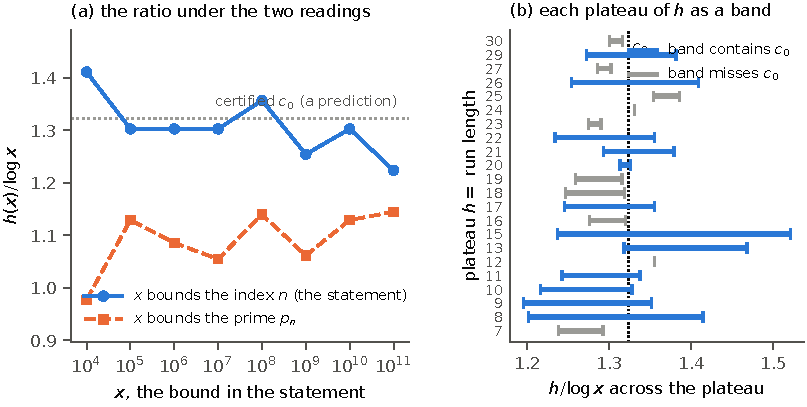
\includegraphics[width=\linewidth]{fig/erdos852-readings.pdf}
\caption{(a) $h(x)/\log x$ by decade under the two readings of the statement, with the certified $c_0$ as a dotted reference: a prediction, drawn differently from the measurements. (b) Each closed plateau of $h$ as the band of $h/\log x$ it occupies, from its start (right end) to its end (left end); the dotted line is $c_0$. Drawn from \texttt{certs/erdos852-h-records.json} through the module the report page uses.}\label{fig:readings}
\end{figure}

\begin{table}[h]\centering\small
\begin{tabular}{lrrrrr}\toprule
$x$ & $h(x)$, index reading & $h/\log x$ & $h(x)$, prime reading & $h/\log x$ & $c_0\log x$\\\midrule
\ReadingRows
\bottomrule\end{tabular}
\caption{The same exact record data under the two readings of ``for some $n<x$''. The last column is the thread's prediction, $c_0\log x$ with the certified $c_0$.}\label{tab:readings}
\end{table}

Sampling at decades has a bias the figure removes. $h$ is a step function whose records are its jumps, so quoting $h/\log x$ at the records reads only the tops of the steps. Between one record closing and the next, $h$ is constant while $\log x$ grows, and the ratio falls from a high at the start of the plateau to a low at its end; each closed plateau is therefore reported as the band it occupies (Table~\ref{tab:records}, Figure~\ref{fig:readings}(b)), and the honest question is whether $c_0$ lies inside the band. It does in \BandsInside{} of \BandsClosed{} closed plateaus from $h=\BandsMinLen$ on; of the misses, \BandsBelow{} bands lie wholly below $c_0$ and \BandsAbove{} wholly above, \BandsAboveShort{} of the latter being plateaus of only \BandsAboveShortIndices{} indices. The misses are shown, not smoothed.

What the comparison says must be stated with the same care as the verdicts. First, the two readings agree asymptotically: $\log p_n=\log n+\log\log n+O(1)$, so a ratio that tends to $c_0$ under one reading tends to $c_0$ under the other, and the data cannot distinguish the two limits. What they distinguish is finite-range behaviour: at the last record the factor $\log n/\log p_n$ is \LogRatioLast, and it tends to $1$ only like $1-\log\log p_n/\log p_n$, which is \LogLogOverLogLast{} there and decays as slowly as anything in analytic number theory. Second, the agreement under the index reading is consistency, not confirmation: eight decades and twenty-two plateaus are evidence about a conjecture that the problem page rightly says no finite computation can settle, and a second-order term of either sign could move the finite-range ratio by the amounts seen. What can be said is this: under the reading the statement gives, the ratio is already flat at the certified constant across everything computed, and under the other reading it is not; and Erd\H{o}s's own question, whether $h(x)=o(\log x)$, is answered by these data in the direction of ``no'' as far as they reach, with the ratio neither decaying nor drifting. The thread's conjecture is recorded in the repository's formal statement of the problem in Lean (which formalises the index reading and states the boundedness of the run-length set as the named side-condition it is, since the supremum of an unbounded set is junk in Mathlib) precisely because it is incompatible with a ``yes''.

\section{A taxonomy of failure, for people who grade mathematics}\label{sec:taxonomy}

The $\Cstar$ episode is the type specimen of a failure class, and the repository's records now hold three distinct classes, each decided, each with the detector that decides it. They are worth naming because the usual defences --- rerun it, cross-check the digits, add compute --- decide none of them.

\begin{enumerate}
\item\emph{The artifact posted as truth.} The computation is silently wrong and its output is stable: every naive rerun reproduces the same digits, two independent float implementations agree with each other, and raising the loop bound changes nothing (Proposition~\ref{prop:mechanism}). The posted value is the bug, printed, with \CstarPubDecimals{} decimals of confidence when \CstarCorrectDecimals{} were real. What decides it is an exact arbiter the value provably lies outside.
\item\emph{The true computation under a false printed claim.} The numerics were right; the posted identity is not what they computed. The repository's specimen is a row of a Ramanujan Machine results sheet whose own polynomials converge to $2/(2\zeta(5)-2\zeta(3)+1)$ while the printed formula carries $-1$, a sign slip, with the printed convergent contradicting the row's own recurrence \cite{RepoRM}. There is no second number to check digits against; what decides it is deciding the printed identity against a certified enclosure of the object the row defines, and then certifying the corrected identity on the same enclosure, so that the mechanism is proved rather than guessed.
\item\emph{The coincidence that survives every screen.} Nothing was computed wrongly; the world contains near-misses deeper than any float. The repository's specimen is a published OEIS constant that agrees with $1/5$ to more significant digits than any decimal screen ever used to announce a discovery has asked for, and is not $1/5$ \cite{RepoImp}. Probability arguments certify confidence, not truth; what decides it is an exact refutation at the full published precision, the only test with a zero false-accept rate.
\end{enumerate}

What the three share: the failure is invisible from inside floating point, stable under repetition, and dressed as precision. For anyone building evaluations or verifiable-reward environments on mathematical ground truth, three consequences follow. Digit-matching ground truth inherits the failure class of whatever computed it: if a reference value came from a float pipeline, class~1 lives inside the answer key, and a model that reproduces the artifact grades as correct --- the reference must carry its own certificate, not just its digits. Human graders cannot decide this class either; no reviewer evaluates a product of \CstarPrimes{} factors by eye, and the $\Cstar$ decimal sat on a public thread from \ThreadDateConstants{} until the correction of \ThreadDateCorrection{} \cite{Thread852}. And a verifier is trustworthy only if it can be shown failing: every instrument here ships controls that must fire (\BatteryReds{} in the battery of \BatteryChecks{} checks, \VerifierReds{} in the stdlib verifier, three forged variants rejected by the Lean kernel) and calibrations against known answers that must pass before any novel claim is decided. An answer key that has never rejected a plausible forgery has an unknown false-accept rate.

\section{What is not claimed}

Nothing asymptotic is proved. The problem page states that 852 cannot be resolved by a finite computation, and this paper agrees: Observation~\ref{obs:readings} is consistency over a finite range, and Section~\ref{sec:readings} says why a finite range cannot separate the two readings' limits. The minimality statements of Proposition~\ref{prop:scan} rest on one exhaustive scan and are not independently re-proved; the existence statement of Theorem~\ref{thm:record} is. The correction of $\Cstar$ concerns the numerical value only: it does not touch the structure of the thread's conditional argument, and since $\tfrac12+\Cstar$ changes in its \CstarDiffDecimal{}th decimal the qualitative conclusion $I_0(c)+J(c)<1$ for small $c>0$ is unaffected; the thread's sieve bounds are quoted as recorded and were not re-derived here. The mechanism identifies a computation, not an author: it says what arithmetic produced the posted digits, not who ran it or what tool proposed it, and the posted $c_0$ is correct to the places it was given. The repository's stack and this paper share an author, which is why the refutation is also carried by a stdlib verifier and by a kernel that is not ours; the enclosures of Theorems~\ref{thm:c0} and~\ref{thm:cstar} beyond the refutation inequality rest on the directed-rounding layer and its battery, and an outside re-derivation of them at the stated widths is invited.

\cmrepro{\setlength{\emergencystretch}{3em}The detached certificate, \path{certs/erdos852-certificate.json}, was exported by \path{tools/export-erdos852-certificate.js} at commit \texttt{\CertGit}; the command
\begin{center}\texttt{python3 tools/verify\_erdos852.py certs/erdos852-certificate.json --sources corpus/sources}\end{center}
re-decides both constants in \VerifierSeconds{}~s with the standard library only. The instrument is \path{instruments/erdos852/} over \path{instruments/bigfloat/}, with \path{families/erdos852-constants.js} as the four objects; its battery (\path{instruments/erdos852/battery.js}, run with \texttt{node}) has \BatteryChecks{} checks. The kernel bridge is \path{lean/erdos852/}; \texttt{bash lean/erdos852/check.sh} builds it and must see the three forgeries rejected. The record scan is \path{instruments/erdos852h/h.js} (\texttt{node instruments/erdos852h/h.js 5e11} reproduces \path{certs/erdos852-h-records.json} in about \HMinutes{} minutes), its analysis \path{analyse.js}, and
\begin{center}\texttt{node instruments/erdos852h/verify-record.js \ExtPrimeRaw{} \ExtLen}\end{center}
re-proves Theorem~\ref{thm:record}. Sources are pinned by SHA-256 in \path{corpus/sources/PINS.json}: the problem page and thread fetched on \ThreadFetchDate, the thread snapshot of \ThreadSnapshotDate{} showing the correction, and the four OEIS entries. The macros of this document are written by \texttt{node tools/paper-numbers/erdos852.js}, which re-hashes every pin, re-runs the naive product, the exact-integer refutation, the battery and the verifier, re-proves the record, and refuses when a record no longer says what a sentence needs; the figure is drawn by \path{tools/paper-numbers/erdos852-fig.py} from the data that script derives. The report pages are \url{https://carlostoledo.co/reports/erdos852.html} and \url{https://carlostoledo.co/reports/erdos852-h.html}; repository commit \texttt{\RepoCommit}.\par}

\begin{thebibliography}{99}\small
\bibitem{Bloom852} T.~F.~Bloom, Erd\H{o}s Problem \#852, \url{https://www.erdosproblems.com/852}, accessed \PageAccessed{} (the page's recommended citation form); pinned as \texttt{corpus/sources/erdos852\_page.html}.
\bibitem{Er85c} P.~Erd\H{o}s, the 1985 source paper keyed [Er85c] on the problem page \cite{Bloom852}, where the bibliographic entry is recorded; not re-verified here.
\bibitem{Thread852} Discussion thread of Erd\H{o}s Problem \#852, \url{https://www.erdosproblems.com/forum/discuss/852}: the comments of \ThreadDateConstants{} (D.~Turturean; P.~Chojecki) stating the conjecture and the two constants, and the correction of \ThreadDateCorrection; snapshots pinned in \texttt{corpus/sources/} (\ThreadCommentsBefore{} comments on \ThreadFetchDate, \ThreadCommentsAfter{} on \ThreadSnapshotDate).
\bibitem{OEIS} OEIS Foundation Inc.\ (2026), The On-Line Encyclopedia of Integer Sequences, \url{https://oeis.org}: A053597, A078515, A079889 (N.~J.~A.~Sloane, 2003, with terms by R.~G.~Wilson~v, K.~Brockhaus, D.~Reble and D.~Johnson, 2002--2012) and A079007 (L.~Elemer, 2002, extended to 2012); entries pinned as \texttt{corpus/sources/oeis\_A0*.txt}.
\bibitem{Lewin81} L.~Lewin, Polylogarithms and Associated Functions, North-Holland, New York, 1981.
\bibitem{IEEE754} IEEE Standard for Floating-Point Arithmetic, IEEE Std 754-2019, IEEE, 2019.
\bibitem{HardyWright} G.~H.~Hardy and E.~M.~Wright, An Introduction to the Theory of Numbers, 6th ed., Oxford University Press, 2008.
\bibitem{Kahan65} W.~Kahan, Further remarks on reducing truncation errors, Comm.\ ACM 8 (1965), 40.
\bibitem{Higham93} N.~J.~Higham, The accuracy of floating point summation, SIAM J.\ Sci.\ Comput.\ 14 (1993), 783--799.
\bibitem{Jaeschke93} G.~Jaeschke, On strong pseudoprimes to several bases, Math.\ Comp.\ 61 (1993), 915--926.
\bibitem{Lean4} L.~de Moura and S.~Ullrich, The Lean 4 theorem prover and programming language, in: Automated Deduction -- CADE 28, Lecture Notes in Computer Science 12699, Springer, 2021, 625--635.
\bibitem{Mathlib} The mathlib Community, The Lean mathematical library, in: Proceedings of the 9th ACM SIGPLAN International Conference on Certified Programs and Proofs (CPP 2020), ACM, 2020, 367--381.
\bibitem{Repo} C.~Toledo, cert-machine: independent exact certification of machine-generated mathematics, \url{https://github.com/carlostoledo1891/cert-machine}, concept DOI 10.5281/zenodo.22225860; the report pages are named in the reproduction section.
\bibitem{RepoRM} The Ramanujan Machine results sheets, re-decided: \url{https://carlostoledo.co/reports/rm-audit.html}, as recorded in the repository \cite{Repo} (family \texttt{families/ramanujan-audit.js}, rows \texttt{rm-zo-z5z3b-printed} and \texttt{-corrected}).
\bibitem{RepoImp} The impostor catalogue: \url{https://carlostoledo.co/reports/impostors.html}, as recorded in the repository \cite{Repo} (A271880 against $1/5$).
\end{thebibliography}

\end{document}
